\section{Pre-processing}
Innanzitutto si è scelto di utilizzare il campo \textit{text} e di escludere il campo \textit{summary}, poiché come visto anche nel esplorazione dei dati questo campo prevede descrizioni troppo brevi e sommarie al fine di identificare degli aspetti.

Prima di passare il testo delle recensioni in input ai modelli vengono fatte le seguenti operazioni di preprocessing. Per prima cosa vengono rimossi gli URL tramite un'espressione regolare. 

Poi vengono rimossi i tag HTML e sostituite le HTML entities (e.g. \textbackslash amp; $\rightarrow$ $\&$). Eventuali frasi o elenchi attaccati vengono separate aggiungendo uno spazio dopo punti e virgole. Successivamente i seguenti caratteri ``+'', ``-'', ``\_'', ``/'', ``\textbackslash'' vengono separati con uno spazio per dividere parole attaccate e vengono rimossi gli spazi in eccesso. Le contrazioni (e.g. i'm $\rightarrow$ I am) e gli slang (e.g. gotta $\rightarrow$ got to) vengono risolti.

Dopo queste operazioni il testo viene diviso in token mantenendo le frasi. In ogni frase viene 
identificato il POS associato ad ogni token che verrà usato per la lemmatization e vengono identificate le negazioni.

Per ogni token vengono rimossi i caratteri non alfanumerici e le ripetizioni (e.g. ``greeeat'' $\rightarrow$ ``greeat'', `gooood' $\rightarrow$ ``good'') tramite espressioni regolari. I token vengono trasformati in minuscolo e poi viene applicato stemming o lemmatization. 

Per le operazioni di preprocessing viene usata la libreria NLTK. Per lo stemming è stato
usato \textit{Snowball Stemmer}, per la lemmatization è stato usato \textit{WordNet Lemmatizer}, come POS tagger è stato usato \textit{Averaged Perceptron Tagger} e per la tokenization il \textit{NLTKWordTokenizer}.

Le stopwords e i token con lunghezza pari a 1 o maggiore di 20 vengono rimossi. Le stopwords usate sono l'unione di quelle usate nelle librerie NLTK e SpaCy.

Ai token precedentemente identificati come negativi viene prefissato ``not\_''. Come mostrato 
nella figura \ref{fig:tokens-example} vengono negati tutti i token che seguono un token identificato
come negativo. Nell'esempio il risultato non è quello desiderato poichè ``speed is pretty good'' non dovrebbe essere negato. Per migliorare questo risultati si potrebbe cambiare il modo di 
dividere le frasi.

\begin{figure}[ht]
    \centering
    
    \begin{quote}
    \begin{mdframed}
        \textbf{Text:} This is a decent tablet for the price, i had no issues with this tablet, speed is pretty good [...]
        
        \textbf{Tokens:}
        [decent tablet price] [not\_issue not\_tablet] [not\_speed not\_pretty not\_good] [...]
      
    \end{mdframed} 
    \end{quote}
    
    \caption{Esempio della negazione dei token con lemmatization.}
    \label{fig:tokens-example}
\end{figure}

% TODO: prove ... lemmatization, stemming, raw

Dopo aver ottenuto i token è stata effettuata una rimozione in base alla \textit{document frequency}.
Sono stati rimossi i token presenti in più del 90\% dei documenti e quelli presenti in meno di 4 documenti, 
mantenendo i token usati come seed (Tabella \ref{tab:rare-tokens}).

\begin{table}[ht]
\resizebox{\textwidth}{!}{%
\begin{tabular}{|l|c|c|c|c|}
\hline
\multicolumn{1}{|c|}{\textbf{Normalization}} &
  \textbf{\begin{tabular}[c]{@{}c@{}}Tokens \\ before removal\end{tabular}} &
  \textbf{\begin{tabular}[c]{@{}c@{}}Tokens in more than \\ 90\% documents\end{tabular}} &
  \textbf{\begin{tabular}[c]{@{}c@{}}Tokens in less than \\ 4 documents\end{tabular}} &
  \textbf{\begin{tabular}[c]{@{}c@{}}Tokens \\ after removal\end{tabular}} \\ \hline
Raw           & 30456 & 0 (0\%) & 19740 (65\%) & 10716 \\ \hline
Lemmatization & 25192 & 0 (0\%) & 16688 (66\%) & 8504  \\ \hline
Stemming      & 20633 & 0 (0\%) & 13145 (64\%) & 7488  \\ \hline
\end{tabular}%
}
\caption{Numero di token prima e dopo la rimozione in base alla \textit{document frequency} al variare della normalizzazione.}
\label{tab:rare-tokens}
\end{table}

% TODO: commenti sulla scelta dei parametri 0.9, 4...

Nella figura \ref{fig:tokens} vengono mostrati i 25 token più frequenti al variare della normalizzazione: raw, lemmatization e stemming.

\begin{figure}[ht]
    \centering
    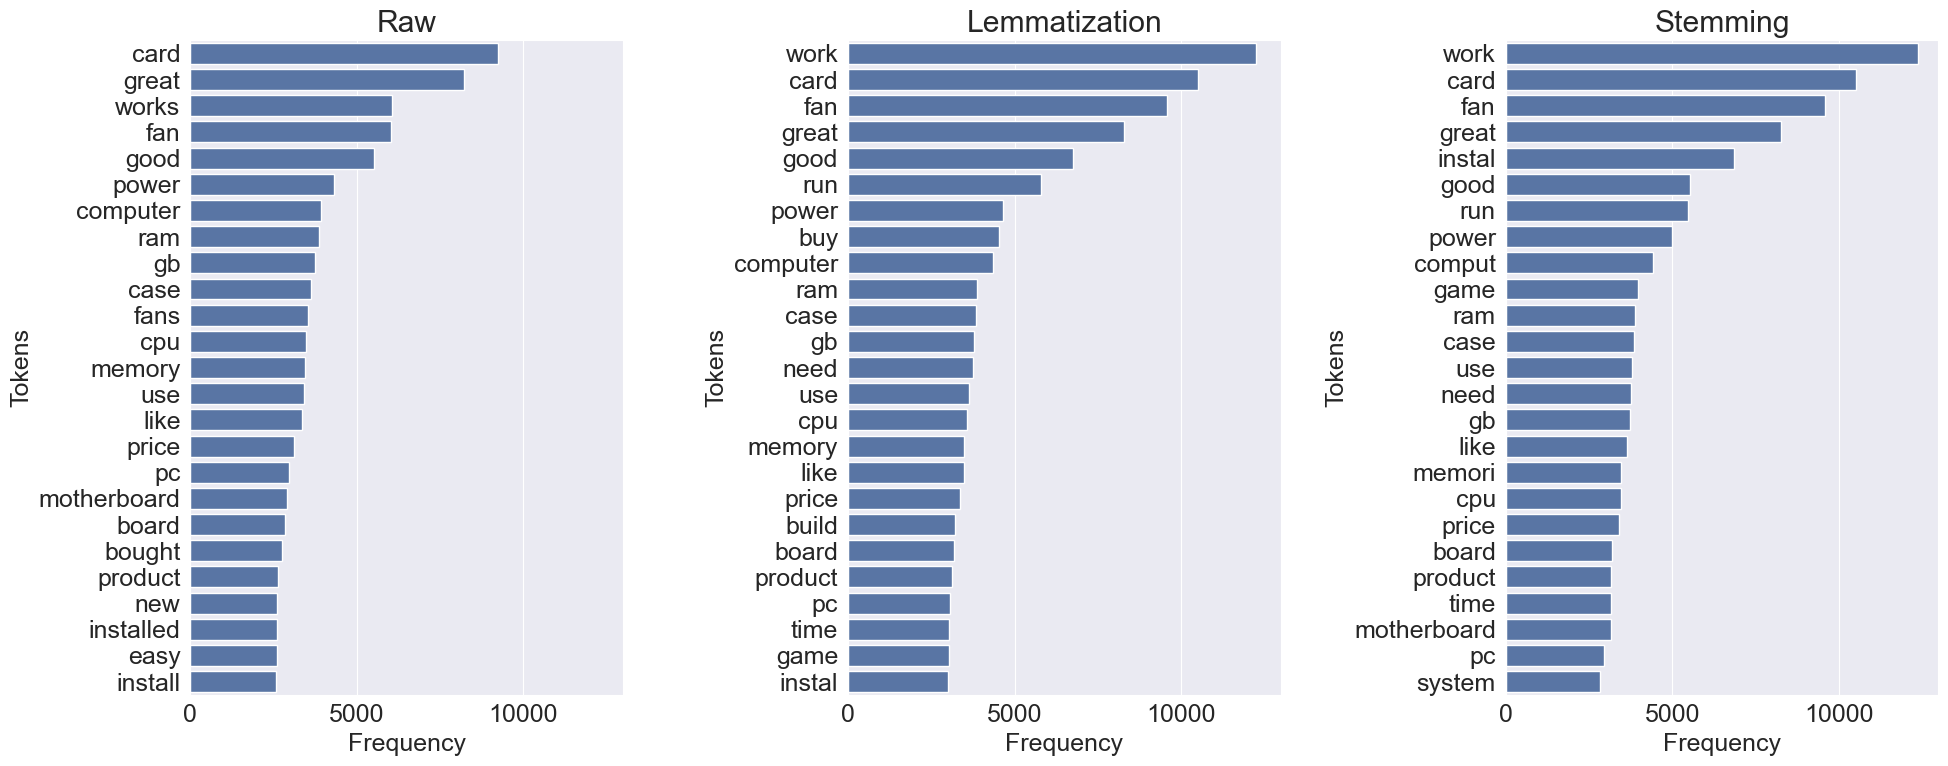
\includegraphics[width=\textwidth]{images/tokens}
    \caption{Top 25 token più frequenti al variare della normalizzazione.}
    \label{fig:tokens}
\end{figure}

Infine come effettuato anche nel lavoro originale di ASUM le frasi con numero di token superiore a 50 vengono ignorate.
